Our system is a \textbf{Centralized Network}, consisting of \emph{N} nodes connected to a hub,
the number of nodes \emph{N} are given from external file. This topology is, also, referred to as \emph{star network}. Since, we use \emph{full-duplex} communication, then each \textbf{node} acts as a sender and a receiver at the same time, sending data and acknowledges \emph{(piggybacked)}.
\newline
\newline
The \textbf{hub} has the following functionalities:
\begin{itemize}
    \item Allocate sessions between nodes.
    \item Navigate packets and acknowledges between peers.
    \item It's considered the control device of access medium, so it's responsible for the different types of channel noise.
    \item Gather the required statistics for each node.
\end{itemize}

\begin{figure}[H]
    \centering
    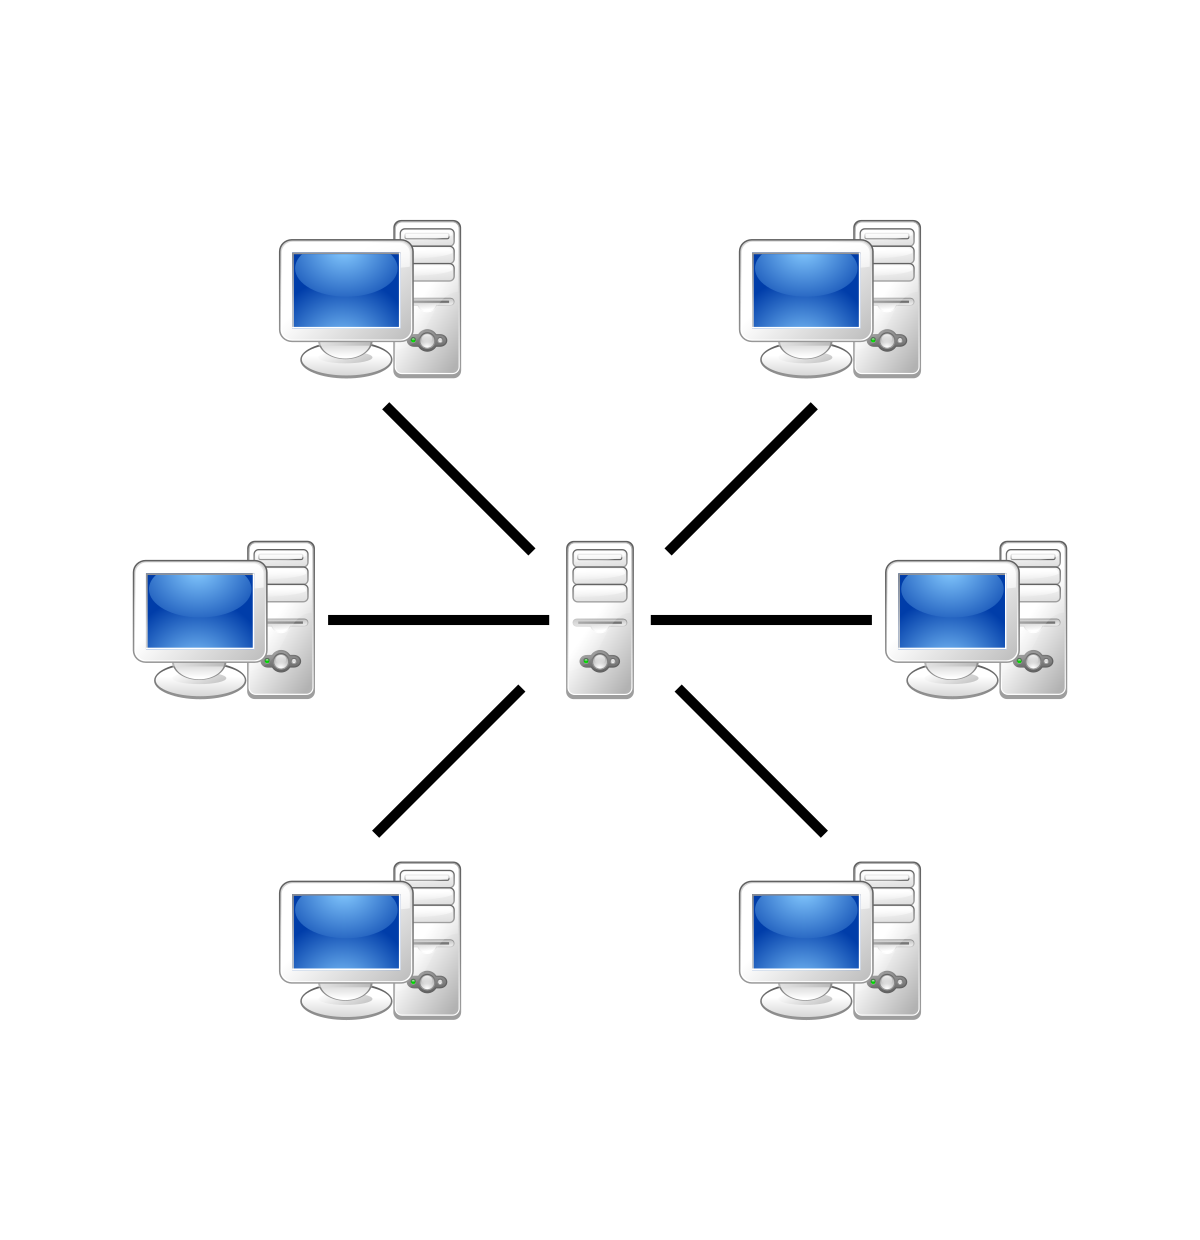
\includegraphics[width=0.6\textwidth]{images/net.png}
    \caption{Centralized Star Network.}
    \label{fig:consoles}
\end{figure}